\appendix
\label{Anhang}
\section{Anhang}

\subsection{Weitere Aktivierungsfunktionen}\label{anhang:weitereaktivierungsfunktionen}

\begin{figure}[h]
    \center
    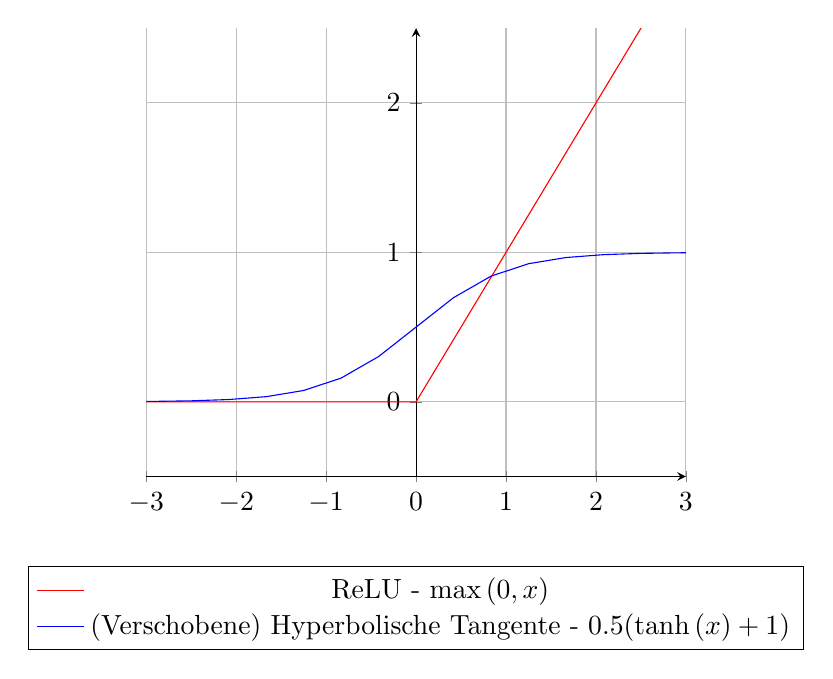
\begin{tikzpicture}
    \begin{axis}
        [
            grid=major,
            xmin=-3,
            xmax=3,
            axis x line=bottom,
            ytick={0,1,2},
            ymax=2.5,
            ymin=-0.5,
            axis y line=middle,
            legend style={at={(0.5,-0.2)},anchor=north}
        ]
        \addplot[red,mark=none]{(x>=0)*x};
        \addplot[blue, mark=none]{0.5*(tanh(\x)+1)};
        \legend{ReLU - $\max{(0,x)}$, (Verschobene) Hyperbolische Tangente - $0.5(\tanh{(x)}+1)$}
    \end{axis}
\end{tikzpicture}
    \caption[Aktivierungsfunktionen]{Weitere Aktivierungsfunktionen, ergänzend zu der Sigmoid Funktion aus Kapitel \ref{funktionsweise}}
    \label{Aktivierungsfunktionen}%
\end{figure}

Die ReLU (Rectified linear Unit) Funktion ist im Vergleich zu anderen Aktivierungsfunktionen, wie der Sigmoidfunktion oder der Hyperbolischen Tangente, deutlich simpler, was sich in Leistungsansprüchen des Trainingsprozesses wiederspiegelt.\footnote{\cite{nnfs}}

\subsection{Code für das Beispiel aus \ref{funktionsweise}}\label{anhang:colab1}

\begin{listing}[H]
    \begin{minted}[fontsize=\footnotesize,linenos]{python}
import tensorflow as tf
import tensorflow.keras.layers as layers

numberOfNeuronsInFirstLayer = 16 
numberOfNeuronsInSecondLayer = 16 
numOfEpochs = 5 

mnist = tf.keras.datasets.mnist

(x_train, y_train), (x_test, y_test) = mnist.load_data() # Laden des MNIST
# Datasets und aufteilen in Trainigsdaten und Testdaten

x_train = tf.keras.utils.normalize(x_train, axis=1) # Normalisieren des Datasets
x_test = tf.keras.utils.normalize(x_test, axis=1)

model = tf.keras.models.Sequential() # Erstellen des Neuronalen Netzwerks
model.add(layers.Flatten())
model.add(layers.Dense(numberOfNeuronsInFirstLayer, activation=tf.nn.sigmoid))
# Hinzufügen der Layer
model.add(layers.Dense(numberOfNeuronsInSecondLayer, activation=tf.nn.sigmoid))
model.add(layers.Dense(10, activation=tf.nn.softmax))

model.compile(optimizer='adam',
              loss='sparse_categorical_crossentropy',
              metrics=['accuracy']) # Kompilieren der Layer zu einem
                                    # trainierfähigen Modell

model.fit(x_train, y_train, epochs=numOfEpochs)
# Trainieren des Modells mit den Trainingsdaten und x Epochen

model.save('beispielModel_MNIST') # Speichern des Modells

    \end{minted}
    \caption{Umsetzung mit Python und Tensorflow}
\end{listing}
Ein interaktives Beispiel gibt es zusätzlich hier in meinem Colab Notebook: \url{https://bit.ly/34Ggfuh}\footnote{Ungekürzter Link: \url{https://colab.research.google.com/drive/1ty_QQlL038YT6KpBjSdqGvIGyH0YXwxW}}

\subsection{Labelcheck}\label{anhang:labelchecktf}

\subsubsection{Die Siegel/Label}\label{angang:label}

\begin{figure}[H]
    \centering
    \subfloat[\centering Bio nach EG-Öko-Verordnung]{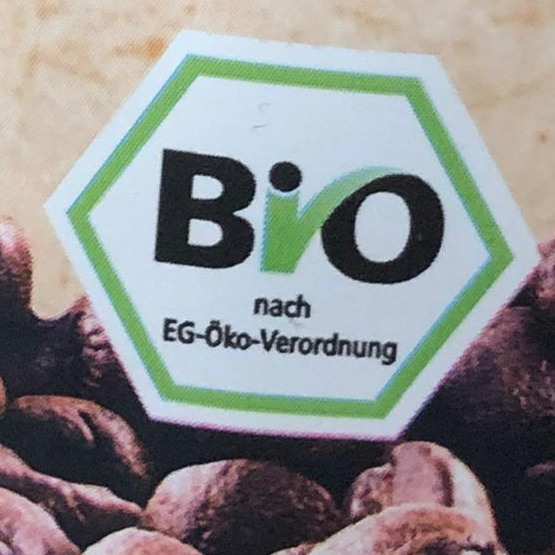
\includegraphics[totalheight=2cm]{bionacheg.jpg}}%
    \qquad
    \subfloat[\centering Bioland]{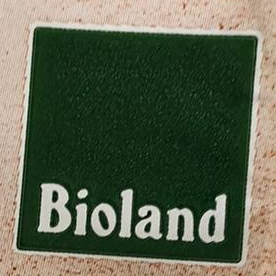
\includegraphics[totalheight=2cm]{bioland.jpg}}
    \qquad
    \subfloat[\centering Demeter]{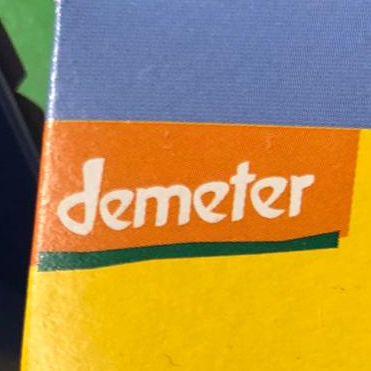
\includegraphics[totalheight=2cm]{demeter.jpg}}
    \qquad
    \subfloat[\centering EU Siegel]{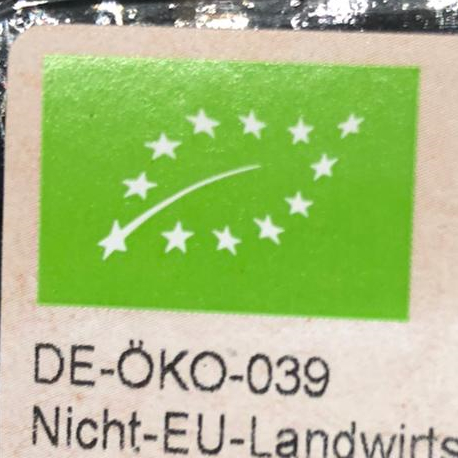
\includegraphics[totalheight=2cm]{eu.jpg}}
    \qquad
    \subfloat[\centering Fairtrade]{
\includegraphics[totalheight=2cm]{fairtrade.jpg}}
    \qquad
    \subfloat[\centering MSC]{
\includegraphics[totalheight=2cm]{msc.jpg}}
    \qquad
    \subfloat[\centering Ohne Gentechnik]{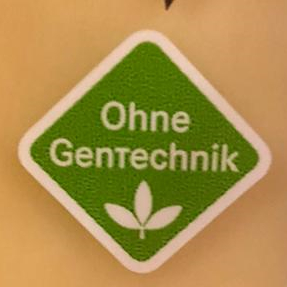
\includegraphics[totalheight=2cm]{ohneGentechnik.jpg}}
    \caption[Label]{Die verschiedenen Label, welche Labelcheck in der Version 1.0 identifizieren kann.}
    \label{labels}%
\end{figure}

\textbf{(a)} Das Produkt enthält keine Farbstoffe, Geschmacksverstärker, künstliche Aromen, Stabilisatoren oder synthetische Süßstoffe. Tiere haben etwas mehr Platz als in konventioneller Tierhaltung und ihre Futtermittel enthalten weder Antibiotika noch Leistungshormone. Gentechnik ist bis 0,9\% erlaubt und es dürfen teilweise weiterhin umweltschädliche Praktiken, zum Beispiel zur Bekämpfung von Pilzen, angewandt werden.\footnote{\cite{egoeko}}

\noindent\textbf{(b)} Für das Bioland Siegel muss der ganze Betrieb biologisch aufgestellt sein und nachweislich Wasser sparen. Ein häufiger Weidegang der Tiere ist vorgeschrieben. Gemüse darf nur auf natürlichem Boden angebaut werden und es darf auch keinerlei Gentechnik angewandt werden. Ebenfalls wird eine recycelbare Verpackung vorgeschrieben.\footnote{\cite{verschiedenelabel}}

\noindent\textbf{(c)} Für das Demeter Siegel müssen mindestens 90\% der Zutaten ebenfalls das Demeter Siegel tragen, das Produkt darf nur Aromen und Extrakte der namensgebenden Pflanze beinhalten und insgesamt werden bloß 22 Zusatzstoffe zugelassen. Gentechnik ist zudem komplett ausgeschlossen. Allerdings muss jeder Betrieb Tiere halten, allerdings darf keine Enthornung durchgeführt werden und das halten von hornlosen Rassen wird auch unterbunden. Der gesamte Betrieb muss ökologisch wirtschaften.\footnote{\cite{verschiedenelabel}}

\noindent\textbf{(d)} Dieses Label gilt in der ganzen EU. Produkte aus dem EU-Ausland müssen die entsprechenden Kriterien erfüllen. Nur noch 44 Zusatzstoffe (anstatt von über 300 in der konventiollen Landwirtschaft) werden geduldet. Dieses Siegel steht allerdings unter starker Kritik, da Betriebe nicht voll auf die ökologische Produktion umgestellt sein müssen, Tiere dennoch mit gentechnisch verändertem Futter gefüttert werden dürfen, und Fleisch-, Blut- und Knochenmehl als Dünger eingesetzt werden darf. Ebenfalls gibt es keine Regelungen zur Einhaltung der Menschenrechte an den Höfen.\footnote{\cite{verschiedenelabel}}

\noindent\textbf{(e)} Das Fairtrade Siegel verspricht humane Arbeitsbedingungen für den Bauern, die Abschaffung von Kinderarbeit, und feste Preise für den Bauern, sodass dieser nicht mehr von den stark schwankenden Weltmarktpreisen abhängig ist. Ebenfalls bieten Fairtrade Produkte die Möglichkeit die Produktionsschritte rückzuverfolgen. Dieses Label hat in Vergangenheit aber auch Kritiken eingesteckt, so dürfen faire und unfaire Zutaten vermischt werden und das Endprodukt darf dennoch das Siegel tragen, wenn auch mit einem gekennzeichneten Mengenausgleich. Auch ist die Preisgestaltung undurchsichtig, so ist das Produkt teilweise deutlich teurer, der Bauer erhält allerdings bei weitem nicht diesen großen Teil.\footnote{\cite{fairtrade}}

\noindent\textbf{(f)} Das MSC Siegel verspricht eine Verhinderung von Überfischung, die Funktionsfähigkeit und Artenvielfalt aller betroffenen Ökosysteme darf nicht beinträchtigt werden und alle regionelen und internationalen Gesetze müssen eingehalten werden. Es gibt aber auch viele Kritiken, so behauptet Greenpeace, MSC würde die Siegel zu früh rausgeben und ein Versprechen an MSC: "in Zukunft wird sich etwas bessern" genüge bereits um die Zertifizierung zu erhalten. Auch dürfen teilweise weiterhin problematische Fangmethoden eingesetzt werden, welche zum Beispiel Schäden am Meeresboden anrichten.\footnote{\cite{msc}}

\noindent\textbf{(g)} Das ohne Gentechnik Siegel unterbindet den Einsatz von gentechnisch veränderten Organismen und Teilen davon, auch Futtermittel wird ohne Gentechnik hergestellt. Ebenfalls wird der Einsatz von gentechnisch veränderten Vitaminen, Aromen, Enzymen und anderen Lebensmittelzusatzstoffen unterbunden.\footnote{\cite{ohneGentechnik}}

\subsubsection{Das Model}\label{anhang:model}

\begin{figure}[H]
    \centering
    \resizebox{!}{\textheight/10*9}{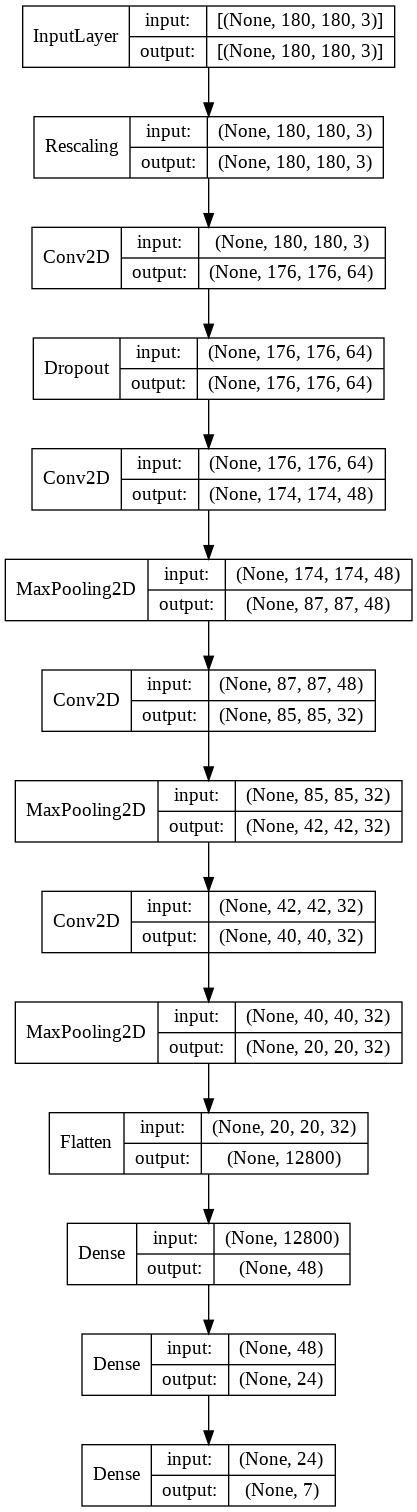
\includegraphics{model2.png}}
    \caption{Visualisierung des Models (Ohne Data Augmentation Layer, siehe \ref{tfcode})}
  \end{figure}

\subsubsection{Code für das Model}\label{tfcode}

\emph{Interaktive Beispiele in meinem Colab Notebook: \url{https://bit.ly/34Ggfuh}\footnote{Ungekürzter Link: \url{https://colab.research.google.com/drive/1ty_QQlL038YT6KpBjSdqGvIGyH0YXwxW}}}. Listing 2,3 und 4 sind ein \textbf{zusammenhängender} Abschnitt, sie passen nur nicht auf eine Seite.

\begin{listing}[H]
    \begin{minted}[fontsize=\footnotesize,linenos]{Python}
import numpy as np
import os
import datetime
import tensorflow as tf
from tensorflow.keras import layers
import tensorboard

batch_size = 16
img_height = 180 # Ich habe mich für 180x180 entschieden um einen Kompromiss
img_width = 180 # zwischen Geschwindigkeit und Genauigkeit einzugehen
data_dir='/content/drive/MyDrive/dataset'
AUTOTUNE = tf.data.AUTOTUNE

train_ds = tf.keras.preprocessing.image_dataset_from_directory(
    # Aufteilen der Daten in Trainingsdaten
    data_dir,
    validation_split=0.22,
    # Das Dataset wird in 78% Trainingsdaten
    # und 22% Validierungsdaten aufgeteilt
    subset='training',
    seed=123,
    image_size=(img_height, img_width),
    batch_size=batch_size)
val_ds = tf.keras.preprocessing.image_dataset_from_directory(
    # und Testdaten
    data_dir,
    validation_split=0.22,
    subset="validation",
    seed=123,
    image_size=(img_height, img_width),
    batch_size=batch_size)

class_names = train_ds.class_names
print('\nClass Names: ' + str(class_names) + '\n') # Ausgeben der Klassen

train_ds = train_ds.cache().shuffle(buffer_size=1000).prefetch(buffer_size=AUTOTUNE)
# I/O Operationen sind in Colab sehr langsam,
val_ds = val_ds.cache().shuffle(buffer_size=1000).prefetch(buffer_size=AUTOTUNE)
# durch die Methoden cache() und prefetch() werden die Daten im RAM gehalten
    \end{minted}
    \caption{Code zum Erstellen und Trainieren des Models aus Labelcheck Teil 1}
\end{listing}

\begin{listing}[H]
    \begin{minted}[fontsize=\footnotesize,linenos]{Python}
model = tf.keras.Sequential([
    layers.experimental.preprocessing.Rescaling(1./255),
    # Normalisieren der Daten, vorher waren die Daten 0-255, jetzt 0-1 /\
    layers.experimental.preprocessing.RandomTranslation(0.1, 0.1),
    # Data Augmentation - Leichte zufällige Veränderungen des
    # Bildes "um das Dataset zu verändern" /\
    layers.experimental.preprocessing.RandomRotation(0.12),
    # Data Augmentation /\
    layers.Conv2D(64, 5, activation='relu'),
    # Convoultional Layer /\
    layers.Dropout(0.1),
    # Lässt Daten aus, hilft gegen Overfitting /\
    layers.Conv2D(48, 3, activation='relu'),
    layers.MaxPooling2D(),
    # Max Pooling Layer /\
    layers.Conv2D(32, 3, activation='relu'),
    layers.MaxPooling2D(),
    layers.Conv2D(32, 3, activation='relu'),
    layers.MaxPooling2D(),
    layers.Flatten(),
    # 2D Layer --> 1D Layer /\
    layers.Dense(48, activation='relu'),
    # Normale Layer /\
    layers.Dense(24, activation='relu'),
    layers.Dense(len(class_names), activation='sigmoid')
    # Output Layer /\
])
    \end{minted}
    \caption{Code zum Erstellen und Trainieren des Models aus Labelcheck Teil 2}\label{teil2}
\end{listing}

\begin{listing}[H]
    \begin{minted}[fontsize=\footnotesize,linenos]{Python}
model.compile(
    optimizer='adam',# Gradient Descent mit Momentum (und mehr)
    loss=tf.losses.SparseCategoricalCrossentropy(from_logits=True),
    metrics=['accuracy'])
    
    logdir = os.path.join("logs", datetime.datetime.now().strftime("%Y%m%d-%H%M%S"))
    tensorboard_callback = tf.keras.callbacks.TensorBoard(logdir, histogram_freq=1)
    
    model.fit(
    train_ds,
    validation_data=val_ds,
    epochs=160,
    shuffle=True,
    callbacks=[tensorboard_callback]
)
    
converter = tf.lite.TFLiteConverter.from_keras_model(model)
# Konvertieren des Keras Models in ein TensorFlow-Lite Model /\
tflite_model = converter.convert()

with open('model.tflite', 'wb') as f: # Speichern des Models
f.write(tflite_model)

tf.keras.utils.plot_model( # Erstellen der Visualisierung des Models
    model, to_file='model.png', show_shapes=True, show_dtype=False,
    show_layer_names=False, rankdir='TD', expand_nested=False, dpi=96
)

# Achtung: Das ist kein Python Code, funktioniert aber in Colab Notebooks
# um das TensorBoard zu öffnen.
# TensorBoard ist eine Web App um den Tainingsprozess zu analysieren
%load_ext tensorboard
%tensorboard --logdir logs
    \end{minted}
    \caption{Code zum Erstellen und Trainieren des Models aus Labelcheck Teil 3}
\end{listing}

\subsubsection{Code für die App}

\emph{Der Code hier ist nicht vollständig, ich habe nur die wichtigsten Teile aufgeführt. Der komplette Code ist unter meinem GitHub Repository \url{https://github.com/phibr0/labelcheck} verfügbar.}

\begin{listing}[H]
    \begin{minted}[fontsize=\footnotesize,linenos]{Dart}
void main() async {
  WidgetsFlutterBinding.ensureInitialized();
  cameras = await availableCameras();
  await Tflite.loadModel(
    model: "assets/model/converted_tflite/model.tflite",
    labels: "assets/model/converted_tflite/labels.txt",
    isAsset: true,
  );
  runApp(MyApp());
}
    \end{minted}
    \caption{Die main Methode von Labelcheck}
\end{listing}

Diese Methode (\mintinline{Dart}{main}) wird beim Start der App aufgerufen, interessant sind hier vorallem Zeilen 3 \& 4, in welchen erstmal alle verfügbaren Kameras in einer Variable gespeichert werden. Dies ist notwendig, da heutzutage viele Smartphones mehrere Kamers verbaut haben. Ab Zeile 4 wird dann TensorFlow-Lite initialisiert\footnote{Die Methoden werden durch das tflite Paket bereitgestellt\cite{tflitepackage}}, indem das Model und die zugehörigen Labels als Parameter übergeben werden. Aufällig ist, dass kein Rückgabewert gespeichert wird. Das liegt daran, dass TensorFlow-Lite platformspezifisch "`unter"' der Flutter Engine liegt und dies automatisch handhabt.

\begin{listing}[H]
    \begin{minted}[fontsize=\footnotesize,linenos]{Dart}
Future<dynamic> classifyImage(String path) async {
    var output = await Tflite.runModelOnImage(
      path: path,
      numResults: 1,
    );
    return output;
}
    \end{minted}
    \caption{Die Methode zum klassifizieren eines Bildes}
\end{listing}

Diese Methode (\mintinline{Dart}{classifyImage}) genügt um eine Klassifizierung durchzuführen. Als einzigen Parameter wird der Dateipfad des Bildes übergeben und dann wird das Bild asynchron klassifiziert, zurückgegeben wird ein Objekt des Typs \mintinline{Dart}{Future<dynamic>}.

\subsection{Die Flutter Architektur}\label{anhang:flutterarc}

\begin{figure}[H]
    \centering
    \resizebox{\textwidth}{!}{
        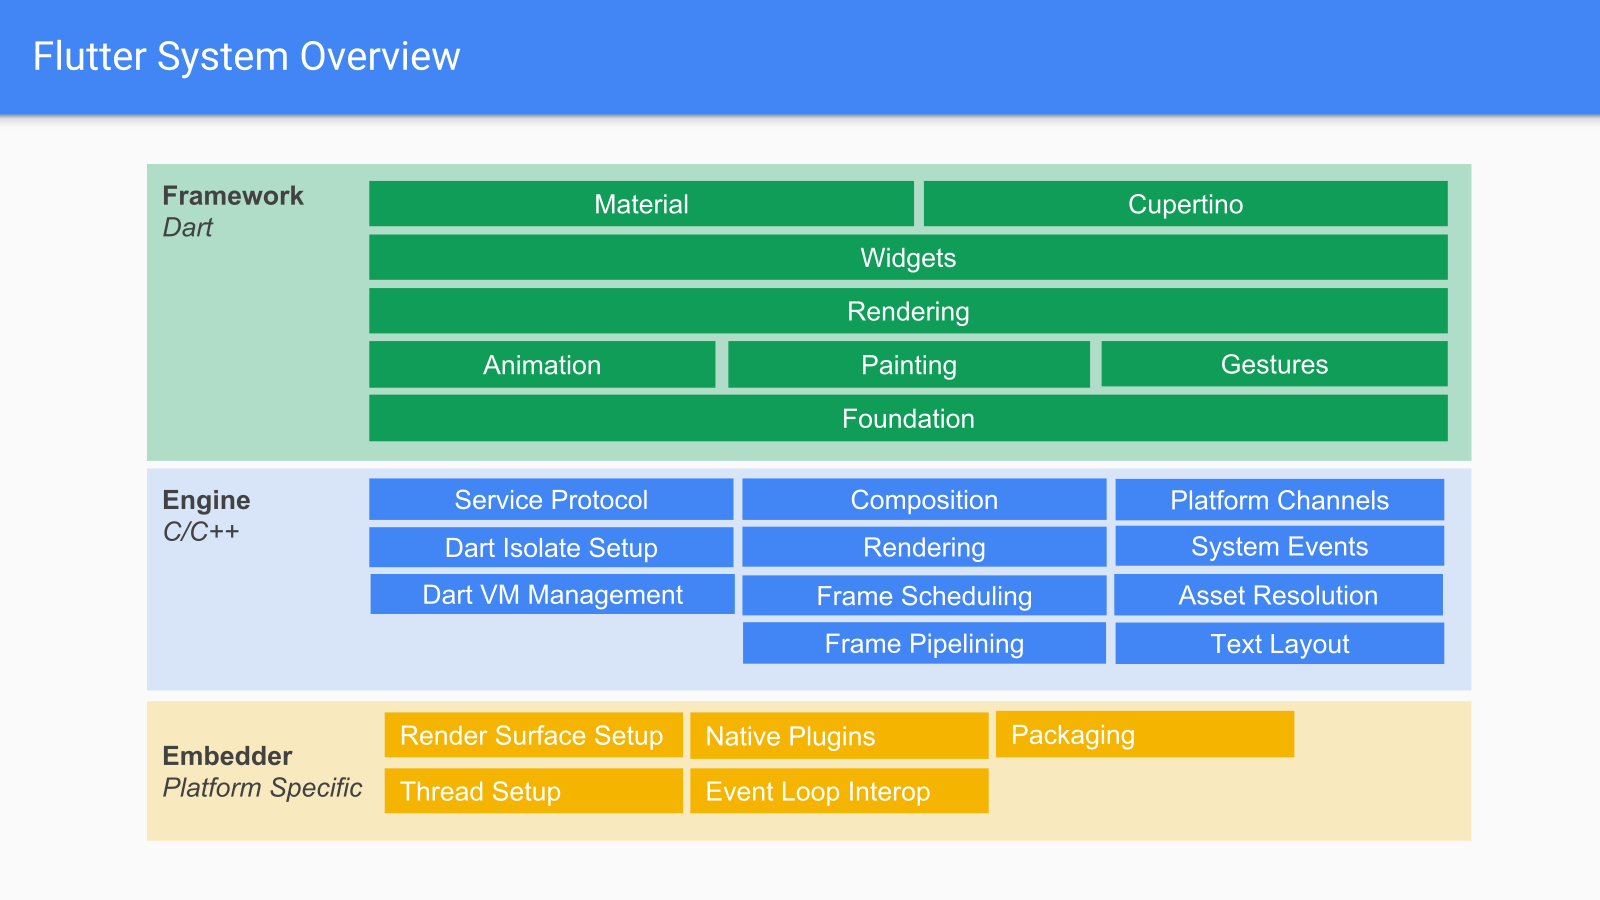
\includegraphics{flutterarchitecture.png}
    }
    \caption{Flutter's Architektur (\cite{flutterarchitecture})}
\end{figure}

Flutters Architektur ist in drei Ebenen unterteilt. Als Basis die "`Embedder Ebene"', welche für jede Platform angepasst werden muss und zum Beispiel für das Thread Management zuständig ist. Dadrüber liegt die "`Engine Ebene"', welche zu einem Großteil in C++ geschrieben ist und zu welcher auch die Grafikengine Skia gehört. Dadrüber liegt die "`Framework Ebene"', welche zum Beispiel die UI Komponenten beinhaltet und komplett in Dart entwickelt wird.\footnote{\cite{flutterarchitecture}}